%pdf-latex
% !TeX program = xelatex
%header nur vom MÜSLI-Vortrag geklaut
% !TEX root = vortrag.tex
% !TEX encoding = UTF-8 Unicode

\documentclass[t, ngerman]{beamer} %compress,

%% Pakete laden...
  \usepackage[T1]{fontenc}
  \usepackage[utf8]{inputenc}
  \usepackage{
      babel,
      bookmark,
      booktabs,
%      blindtext,
      colortbl,
%      eurosym,
      graphicx,
	  hyperref,
%      libertine,
      microtype,
      pifont,
      pgfpages,
      tikz,
%      xspace,
  }


%% Design festlegen...
  \mode<presentation>{
%      \useoutertheme[subsection=false]{smoothbars}
      \useinnertheme{rectangles} % rectangles, circles, rounded
      \usecolortheme[RGB={153,0,0}]{structure}
      \definecolor{unihd}{RGB}{153,0,0}
      \definecolor{dark}{RGB}{115,0,0}
      \definecolor{light}{RGB}{241,229,229}
      \usecolortheme{whale}
		 \usecolortheme{orchid}
%	   \usecolortheme{beaver}
%      \setbeamercovered{transparent}
      \beamertemplatenavigationsymbolsempty
%      \setbeameroption{show notes on second screen}
      \setbeamertemplate{note page}[plain]
      \logo{
\includegraphics[width=3.5cm]{fs-logo-small}}

  }

%% nützliche Definitionen...
  \graphicspath{{media/}}

%% Titelinformationen...
  \title[Studienverwaltung$\mu$]{Das Müsli und das LSF\\\small oder: wer wie was wo Stundenplan}
  \author[
	koebi
  ]{
	Jakob Schnell\\{\scriptsize\url{koebi@mathphys.stura.uni-heidelberg.de}}
  }
%  \institute{  
\includegraphics[width=5.5cm]{fs-logo-big} }

  \date{\vspace*{-2em}\\ 01. Oktober 2018}

  \hypersetup{
      pdfauthor={Jakob Schnell},
      pdftitle={Müsli-Vortrag},
      pdfsubject={hihi},
      pdfkeywords={1},
      pdfpagelayout={SinglePage},
  }
  


\newenvironment{rcases}{%
  \left.\renewcommand*\lbrace.%
  \begin{cases}}%
{\end{cases}\right\rbrace}


\begin{document}

\begin{frame}[fragile]
    \maketitle{}
\end{frame}

\begin{frame}{Inhalt des Vortrags}
    \begin{minipage}[t]{0.515\textwidth}
        \tableofcontents[sections={1-5}]
    \end{minipage}
    \begin{minipage}[t]{0.475\textwidth}
        \tableofcontents[hideallsubsections, sections={6-11}]
    \end{minipage}
\end{frame}

\begin{frame}{Wer will mir hier was erzählen!?}
    \vfill
    \begin{center}
        {\Large Johanna Riedel} \\
        \mail{johanna@mathphys.stura.uni-heidelberg.de} \\
        \vspace{1em}
        {\Large Christian Heusel } \\
        \mail{chris@mathphys.stura.uni-heidelberg.de} \\
    \end{center}
\end{frame}

\begin{frame}{Präambel}
    \Large
    \begin{center}
        \only<1->{
           {\huge \DejaSans{} 😇} Es wird die Folien zum Download geben! {\huge \DejaSans{} 😇}\\[0.7em]
        }
        \only<1>{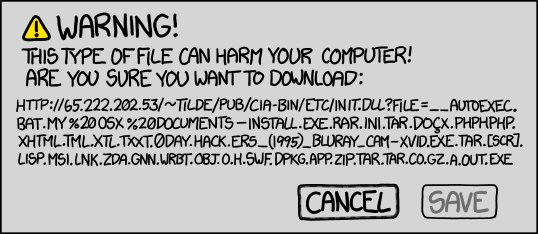
\includegraphics[scale=0.6]{images/xkcd_1.png}}
        \only<2->{
        {\huge \DejaSans{}😏 } Der Vortrag wird auch hochgeladen! {\huge \DejaSans{}😏 } }

        \only<3->{
           {\huge \DejaSans{} 😺} Stellt Fragen, im Währenden oder am Ende! {\huge \DejaSans{} 😺}\\[0.7em]
        }
        \only<4->{
            
\includegraphics[width=0.5\textwidth]{images/lets_go}
        }
    \end{center}
\end{frame}


\section{Digitale Infrastruktur}
\begin{frame}{Übersicht: Digitale Infrastruktur}
    \large
    \begin{itemize}
        \item{WLAN}
        \item{Drucken}
        \item{VPN}
        \item{CIP-Pool}
    \end{itemize}
\end{frame}


%%%%%%%%%%%%%%%%%%%%%%%%%%%%%%%%%%%%%%%%%%%%%%%%%%%%%%%%%%%%
% WLAN
%%%%%%%%%%%%%%%%%%%%%%%%%%%%%%%%%%%%%%%%%%%%%%%%%%%%%%%%%%%%

\subsection{WLAN}
\begin{frame}{Eduroam}
    \begin{minipage}[t]{0.715\textwidth}
        \vspace{-2em}
        \large \textbf{Was ist das Eduroam?}
        \normalsize
        \begin{itemize}
            \item<1-> große Abdeckung in Heidelberg
            \item<2-> Zugang in vielen weiteren Ländern der Welt
            \item<3-> Verschlüsselter Internetzugang
            \item<4-> für den täglichen Gebrauch
        \end{itemize}
        \only<1>{
            \begin{center}
                \vspace{-6.5em}
                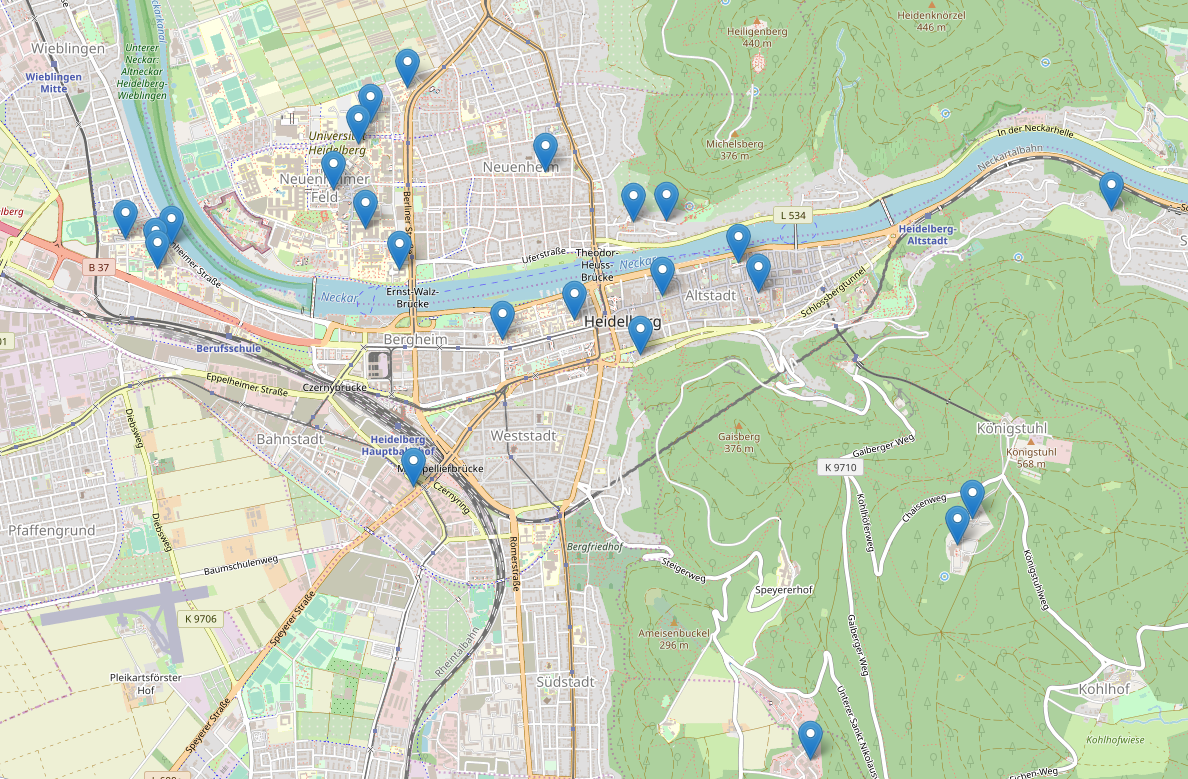
\includegraphics[width=1.3\textwidth]{eduroam_map.png}
            \end{center}
        }
    \end{minipage}
    \begin{minipage}[t]{0.25\textwidth}
        \begin{flushright}
            
\includegraphics[width=0.6\textwidth]{eduroam450pix}
        \end{flushright}
    \end{minipage}
\end{frame}

\begin{frame}{Eduroam einrichten -- leicht gemacht}
    \large \url{https://cat.eduroam.org} \\
    \begin{minipage}[t]{0.515\textwidth}
        \begin{enumerate}
            \item<+-> Link aufrufen
            \item<+-> \glqq{}Uni Heidelberg\grqq{} suchen
            \item<+-> Tool herunterladen
            \item<+-> Tool ausführen
            \item<+-> Zugangsdaten eingeben
            \item<+-> Fertig!
        \end{enumerate}
    \end{minipage}
    \begin{minipage}[t]{0.4\textwidth}
        \vspace{0cm}
        \begin{center}
            \qrcode[height=0.8\textwidth, link]{https://cat.eduroam.org}
        \end{center}
    \end{minipage}
\end{frame}


\begin{frame}{Übersicht: Verfügbare WiFi-Netze}
    \large \textbf{Welche Netze gibt es noch?}
    \normalsize
    \begin{itemize}[<+->]
        \item \texttt{eduroam} \\
            für den täglichen Gebrauch
        \item \texttt{UNI-HEIDELBERG} \\
            Internet nur über VPN, kaum Ports gesperrt
        \item {\color{gray}(\texttt{Heidelberg4You})} \\
            Unsicher, unzuverlässig, funktioniert aber einfach so
        \item {\color{gray}(\texttt{UNI-WEBACCESS})} \\
            Unsicher, für Tagungsgäste
    \end{itemize}
\end{frame}

%%%%%%%%%%%%%%%%%%%%%%%%%%%%%%%%%%%%%%%%%%%%%%%%%%%%%%%%%%%%
% Drucken
%%%%%%%%%%%%%%%%%%%%%%%%%%%%%%%%%%%%%%%%%%%%%%%%%%%%%%%%%%%%

\subsection{Drucken}
\begin{frame}{Drucken}
    \large \textbf{Wie drucke ich denn in der Uni?}
    \normalsize
    \begin{enumerate}
        \item die zu druckende Datei im Web-Portal hochladen \\
            {\footnotesize
                \begin{itemize}
                    \item \url{https://ricoh-eop.urz.uni-heidelberg.de} \\
                    \item \url{https://www.urz.uni-heidelberg.de/de/mobiles-drucken}
                \end{itemize}
            }
        \item zu einem der FollowMe-Printer laufen
        \item Studiausweis einstecken
        \item mit der Uni-ID anmelden
        \item Dokumente ausdrucken
    \end{enumerate}
\end{frame}

%%%%%%%%%%%%%%%%%%%%%%%%%%%%%%%%%%%%%%%%%%%%%%%%%%%%%%%%%%%%
% VPN
%%%%%%%%%%%%%%%%%%%%%%%%%%%%%%%%%%%%%%%%%%%%%%%%%%%%%%%%%%%%

\subsection{VPN}
\begin{frame}{Was ist denn VPN?}
    \large
    \begin{itemize}
        \item \textbf{V}irtual \textbf{P}rivate \textbf{N}etwork
        \item Ein VPN ermöglicht den (Fern-)Zugriff auf andere Netze
        \item Alle Daten werden für den Transport verschlüsselt
        \item hat erstmal nichts mit einem VPN Anbieter zu tun \\
              (NordVPN, TunnelBear, ExpressVPN)
    \end{itemize}
\end{frame}

\begin{frame}{Wozu nützt mir ein VPN?}
    \large
    \begin{itemize}
        \item sichere Verbindung (z.B. falls man im FlixBus o.ä. ist)
        \item man ist \glqq{}virtuell\grqq{} im Uni Netz (z.B. Passwort ändern, UB)
        \item man ist damit auch in Deutschland \\
            (z.B. Mediathek, (legales) Streaming)
        \item Nutzung von WLAN/Ethernet-Dosen
    \end{itemize}
    Download Link: \\
    {\normalsize \href{https://vpnsrv0.urz.uni-heidelberg.de/+CSCOE+/logon.html}{\texttt{vpnsrv0.urz.uni-heidelberg.de/+CSCOE+/logon.html}}}
\end{frame}

\begin{frame}{Wie sieht das aus?}
    \begin{center}
        \only<1>{%
            \vspace*{-1.1cm}
            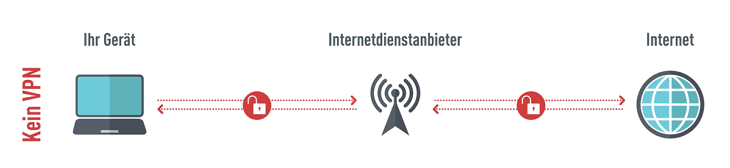
\includegraphics[scale=2.3]{images/vpn_1.png}
        }
        \only<2>{%
            \vspace*{-0.7cm}
            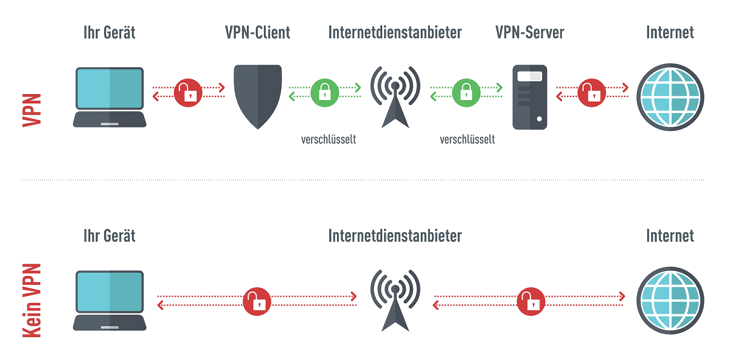
\includegraphics[scale=2.3]{images/vpn.png}
        }
    \end{center}
\end{frame}

%%%%%%%%%%%%%%%%%%%%%%%%%%%%%%%%%%%%%%%%%%%%%%%%%%%%%%%%%%%%
% CIP-Pool
%%%%%%%%%%%%%%%%%%%%%%%%%%%%%%%%%%%%%%%%%%%%%%%%%%%%%%%%%%%%

\subsection{CIP-Pool}
\begin{frame}{CIP-Pool}
    \large
    \textbf{Es gibt verschiedene CIP-Pools:}
    \begin{itemize}
        \item Mathematikon Bibliothek (INF 205)
        \item Universitätbibliothek in der Altstadt
        \item \textcolor{gray}{Universitätsrechenzentrum (INF 293)}
        \item \textcolor{gray}{Kichhoff Institut für Physik (INF 227)}
    \end{itemize}
\end{frame}

\section{Das LSF}
\begin{frame}{Das LSF --- Lehre, Studium und Forschung}

    \large \url{https://lsf.uni-heidelberg.de} \\
    \begin{minipage}[t]{0.515\textwidth}
        \begin{itemize}
            \item{Veranstaltungssuche}
            \item{Studienbescheinigung}
            \item{Rückmeldung}
            \item{Bafög-Daten}
            \item{Noten}
            \item{Stundenplan}
        \end{itemize}
    \end{minipage}
    \begin{minipage}[t]{0.4\textwidth}
        \vspace{0.4cm}
        \begin{center}
            \qrcode[height=0.65\textwidth, link]{https://lsf.uni-heidelberg.de}
        \end{center}
    \end{minipage}
\end{frame}

\begin{frame}{Das LSF --- Lehre, Studium und Forschung}
    \vspace{6em}
    \begin{center}
        \Large Eine Tour durch das LSF findet ihr im hochgeladenen Vortragsvideo!
    \end{center}
\end{frame}


\section{Das MÜSLI}
\begin{frame}{MÜSLI --- \normalsize Mathematisches Übungsgruppen- und Scheinlisten-Interface}

    \large \url{https://muesli.mathi.uni-heidelberg.de/}

    \begin{minipage}[t]{0.7\textwidth}

    \begin{itemize}
        \item Eintragung in Übungsgruppen
        \item Einsehen von Zettelpunkten
        \item E-Mail-Adressen der Tutor*innen
        \item Klausuranmeldung
        \item Noten
    \end{itemize}
    \end{minipage}
    \begin{minipage}[t]{0.28\textwidth}
        \vspace*{0em}
        \begin{center}
            \qrcode[height=0.9\textwidth]{https://muesli.mathi.uni-heidelberg.de/}
        \end{center}
    \end{minipage}
\end{frame}

\begin{frame}{MÜSLI --- \normalsize Mathematisches Übungsgruppen- und Scheinlisten-Interface}
    \vspace{6em}
    \begin{center}
        \Large Eine Tour durch das MÜSLIi findet ihr im hochgeladenen Vortragsvideo!
    \end{center}
\end{frame}


%%%%%%%%%%%%%%%%%%%%%%%%%%%%%%%%%%%%%%%%%%%%%%%%%%%%%%%%%%%%
% Universitätsbibliothek
%%%%%%%%%%%%%%%%%%%%%%%%%%%%%%%%%%%%%%%%%%%%%%%%%%%%%%%%%%%%

\section{Unibibliothek}
\begin{frame}{Unibibliothek}
    \only<1>{%
        Welche Bibliotheken gibt es an der Uni?
        \begin{itemize}
            \item \textbf{Institutsbibliotheken}
                \begin{itemize}
                    \item Fachspezifisch
                    \item Normalerweise nur Präsenzbibliotheken, d.h. keine Ausleihe möglich
                    \item Mathe-Info-Bib befindet sich im EG des Mathematikons
                \end{itemize}
            \item \textbf{Zentralbibliotheken}
                \begin{itemize}
                    \item  Nicht fachspezifisch
                    \item Hauptbibliothek in der Altstadt (Plöck 107-109, Ausleihe im EG)
                    \item Zweigstelle im Neuenheimer Feld (Im Neuenheimer Feld 368, Ausleihe im 3.OG)
                \end{itemize}
        \end{itemize}
    }
    \only<2>{%
        Beachtet
        \begin{itemize}
        \item \textbf{Bibliotheksangebot nutzen}
                \begin{itemize}
                    \item Studierendenausweis = Nutzerausweis
                    \item Um alle Angebote nutzen zu können, müsst ihr euren Ausweis freischalten \\
                        \href{https://www.ub.uni-heidelberg.de/service/anmeldung.html}{\texttt{www.ub.uni-heidelberg.de/service/anmeldung.html}}
                \end{itemize}
            \item \textbf{Schließfächer}
                \begin{itemize}
                    \item Zentralbibliotheken: Ihr braucht eine Zwei-Euro-Münze
                    \item Mathe-Info-Bib: Es gibt Schließfächer mit Zahlencodes oder Schlüsseln; Schließfachschüssel erhaltet ihr bei der Bibliotheksaufsicht gegen ein Pfand (z.B. Ausweis)
                \end{itemize}
        \end{itemize}
    }
    \only<3>{%
        Was bieten euch Bibliotheken?
        \begin{itemize}
            \item{\textbf{Lernort:} allein oder zusammen (Gruppenarbeitsräume reservieren: \url{https://www.ub.uni-heidelberg.de/service/gruppenarbeitsraeume.html})}
            \item{\textbf{Literatur}}
                  \begin{itemize}
                        \item{Finden, nutzen, ausleihen und downloaden}
                        \item{Mehr Literatur über Datenbanken finden}
                        \item{Fernleihe}
                        \item{Teilweise Zugriff auf Online-Angebot von Zeitschriften}
                  \end{itemize}
            \item Weitere Informationen (z.B. Führungen und Kurse) \\
                \href{https://www.ub.uni-heidelberg.de/schulung/Welcome.html}{\texttt{www.ub.uni-heidelberg.de/schulung/Welcome.html}}
        \end{itemize}
    }
\end{frame}

\begin{frame}{Unibiliothek --- HEIDI}
    Bibliothekskatolog HEIDI
    \begin{itemize}
        \item \url{https://katalog.ub.uni-heidelberg.de}
        \item Medien finden und ihren Standort in Erfahrung bringen oder downloaden
    \end{itemize}
\end{frame}

\begin{frame}{Unibiliothek --- HEIDI}
    \vspace{6em}
    \begin{center}
        \Large Eine Tour durch HEIDI findet ihr im hochgeladenen Vortragsvideo!
    \end{center}
\end{frame}

\begin{frame}{Vielen Dank fürs Zuhören!}
    \vfill
    \begin{center}
        \Huge Gibt es Fragen? \\[12pt]
        \large Meldet euch einfach oder schreibt eure Frage(n) in den Chat \\[20pt]
        \normalsize \texttt{EDV-Vortrag mit Johanna \& Chris}
    \end{center}
\end{frame}

\end{document}
